\documentclass[11pt,a4paper]{article}
\usepackage[utf8]{inputenc}
\usepackage[T1]{fontenc}
\usepackage[spanish,es-minimal,es-noshorthands]{babel}
\usepackage{lmodern}
\usepackage[sfdefault,lining]{FiraSans}
\usepackage[a4paper,top=2.3cm,bottom=2.2cm,left=1.8cm,right=1.8cm,headheight=1.3cm,headsep=0.4cm,footskip=1cm]{geometry}
\usepackage{amsmath,amssymb}
\usepackage{icomma}
\usepackage{graphicx}
\usepackage[table]{xcolor}
\usepackage{tikz}
\usepackage{fontawesome5}
\usepackage{ccicons}
\usepackage{fancyhdr}
\usepackage{lastpage}
\usepackage{tasks}
\usepackage{needspace}
\usepackage[most]{tcolorbox}
\usepackage{array}
\usepackage[hidelinks]{hyperref}
\AtBeginDocument{\hypersetup{pdftitle={Ficha de ejercicios de la unidad 4: Límites y continuidad. 2º Bach.},pdfsubject={Matemáticas CCSS 2º Bach.},pdfkeywords={límites, límites en el infinito, comparación de infinitos, indeterminaciones, límites laterales, continuidad, funciones a trozos, parámetros, asíntotas, PAU}}}

\definecolor{navy}{HTML}{1B2748}
\definecolor{accent}{HTML}{E8603A}
\definecolor{teal}{HTML}{1F9E90}
\definecolor{soft}{HTML}{EEF1F8}
\definecolor{muted}{HTML}{5D6685}

\setlength{\parindent}{0pt}
\setlength{\parskip}{3pt}
\settasks{label=\alph*), label-format=\bfseries\color{navy}, label-width=1.3em, item-indent=1.8em, column-sep=0.6em, after-item-skip=5pt, before-skip=3pt, after-skip=4pt}

% ---------- capçalera i peu ----------
\newcommand{\llicencia}{\href{https://creativecommons.org/licenses/by-nc-sa/4.0/deed.es}{\ccbyncsa}\ \ Licencia Creative Commons Atribución-NoComercial-CompartirIgual 4.0 Internacional (CC BY-NC-SA 4.0)}
\pagestyle{fancy}
\fancyhf{}
\fancyhead[L]{\raisebox{-0.35\height}{
\includegraphics[height=0.95cm]{logo-gva.png}}}
\fancyhead[C]{\small\color{muted}Ficha de ejercicios · Unidad 4: Límites y continuidad · 2\textsuperscript{o} Bach.}
\fancyhead[R]{\raisebox{-0.35\height}{
\includegraphics[height=0.95cm]{logo-vermellar.png}}}
\fancyfoot[L]{\scriptsize\color{muted}\llicencia}
\fancyfoot[R]{\small\color{muted}\thepage}
\renewcommand{\headrulewidth}{0.4pt}
\renewcommand{\headrule}{\color{muted!40}\hrule height \headrulewidth}
\fancypagestyle{primera}{\fancyhf{}\renewcommand{\headrulewidth}{0pt}
  \fancyfoot[L]{\scriptsize\color{muted}\llicencia}
  \fancyfoot[R]{\small\color{muted}\thepage}}

% ---------- nivells i exercicis ----------
\newcommand{\estrelles}[1]{{\color{accent}\ifcase#1\or\faStar\faStar[regular]\faStar[regular]\or\faStar\faStar\faStar[regular]\or\faStar\faStar\faStar\fi}}
\newcounter{exer}
\newcommand{\ex}[1]{\par\needspace{4\baselineskip}\medskip\refstepcounter{exer}\noindent{\color{navy}\bfseries\theexer.}\ \ }

\newcommand{\seccio}[2]{\par\needspace{10\baselineskip}\bigskip
  \begin{tcolorbox}[colback=navy,colframe=navy,coltext=white,arc=2mm,boxrule=0pt,left=3mm,right=3mm,top=1.2mm,bottom=1.2mm]
  {\large\bfseries #1\quad #2}
  \end{tcolorbox}\vspace{-2pt}}


% quadre de recordatori (només a la fitxa d'exercicis)
\newcommand{\recorda}[1]{\par\smallskip\begin{tcolorbox}[colback=accent!7,colframe=accent!55,arc=2mm,boxrule=0.5pt,left=2.5mm,right=2.5mm,top=1mm,bottom=1mm]\small{\color{accent}\faLightbulb[regular]}\ \textbf{Recuerda:}\ #1\end{tcolorbox}}
% etiqueta dels exercicis de la PAU d'altres comunitats
\newcommand{\pau}[1]{{\color{teal}\small\bfseries\faUniversity\ PAU · #1.}\ }
\newcommand{\res}[1]{#1}\newcommand{\rest}[1]{#1}

% =====================================================================
% Capçalera FentMates de les fitxes: un color per a cada curs.
% Els colors són els de la pàgina inicial (LEVELS a assets/js/materials.js);
% el logo ve de _eines/logo/pdf/ (python3 _eines/logo/genera.py).
%
% Ús, al final del preàmbul de la unitat:
%   % =====================================================================
% Capçalera FentMates de les fitxes: un color per a cada curs.
% Els colors són els de la pàgina inicial (LEVELS a assets/js/materials.js);
% el logo ve de _eines/logo/pdf/ (python3 _eines/logo/genera.py).
%
% Ús, al final del preàmbul de la unitat:
%   % =====================================================================
% Capçalera FentMates de les fitxes: un color per a cada curs.
% Els colors són els de la pàgina inicial (LEVELS a assets/js/materials.js);
% el logo ve de _eines/logo/pdf/ (python3 _eines/logo/genera.py).
%
% Ús, al final del preàmbul de la unitat:
%   \input{../comu/fentmates.tex}
%   \fmcurs{1eso}
% i, al començament del document:
%   \capcalera{Matemàtiques}{1r ESO}{Fitxa d'exercicis · Unitat 2}{Divisibilitat}
% Opcional abans de \input: \def\fmneed{14} (espai mínim abans de cada secció).
% =====================================================================
\makeatletter
\def\fm@logodir{../../logo/pdf}
\providecommand{\fmneed}{10}
\def\fm@cursnom{}

% clau del curs, color i color del text damunt del color
\newcommand{\fm@curs}[3]{\@namedef{fm@color@#1}{#2}\@namedef{fm@text@#1}{#3}}
\fm@curs{1eso}{E6B84A}{navy}
\fm@curs{2eso}{3B82F6}{white}
\fm@curs{3eso}{FF7A50}{white}
\fm@curs{4eso-a}{A78BFA}{white}
\fm@curs{4eso-b}{6D28D9}{white}
\fm@curs{1batx-mi}{9B1C1C}{white}
\fm@curs{1batx-ccss}{EF6B6B}{white}
\fm@curs{2batx-mii}{1E6B47}{white}
\fm@curs{2batx-ccss}{2BB3A3}{white}

\newcommand{\fmcurs}[1]{%
  \@ifundefined{fm@color@#1}{\PackageError{fentmates}{Curs desconegut: #1}{}}{}%
  \edef\fm@tmp{\noexpand\definecolor{curs}{HTML}{\@nameuse{fm@color@#1}}%
               \noexpand\colorlet{curstext}{\@nameuse{fm@text@#1}}}\fm@tmp
  \colorlet{cursfosc}{curs!72!black}%
  \def\fm@logo{\fm@logodir/vertical-#1.pdf}%
  \def\fm@marca{\fm@logodir/marca-#1.pdf}}

% ---------- capçalera de la primera pàgina ----------
% #1 matèria (petit), #2 curs, #3 tipus de document i unitat, #4 títol
\newcommand{\capcalera}[4]{%
  \gdef\fm@cursnom{#2}%
  \par\noindent
  \begin{tcolorbox}[colback=curs,colframe=curs,boxrule=0pt,arc=2.2mm,width=3.5cm,height=2.15cm,
      valign=center,left=3mm,right=2mm,top=1mm,bottom=1mm,nobeforeafter,box align=center]
    \color{curstext}{\footnotesize #1}\par\vspace{1pt}{\fontsize{19}{21}\selectfont\bfseries #2\par}%
  \end{tcolorbox}\hspace{5mm}%
  \begin{minipage}[c]{\dimexpr\linewidth-3.5cm-5mm-2.9cm\relax}
    {\color{cursfosc}\small\bfseries\MakeUppercase{#3}}\par\vspace{2pt}
    {\color{navy}\fontsize{20}{23}\selectfont\bfseries #4\par}
  \end{minipage}\hfill
  \begin{minipage}[c]{2.6cm}\raggedleft\includegraphics[width=2.6cm]{\fm@logo}\end{minipage}\par
  \vspace{2pt}}

% ---------- barres de secció del color del curs ----------
\renewcommand{\seccio}[2]{\par\needspace{\fmneed\baselineskip}\bigskip
  \begin{tcolorbox}[colback=curs,colframe=curs,coltext=curstext,arc=2mm,boxrule=0pt,left=3mm,right=3mm,top=1.2mm,bottom=1.2mm]
  {\large\bfseries #1\quad #2}
  \end{tcolorbox}\vspace{-2pt}}

% ---------- estrelles de dificultat del color del curs (a Batxillerat no se'n posen) ----------
\@ifundefined{estrelles}{}{%
  \renewcommand{\estrelles}[1]{{\color{curs}\ifcase#1\or\faStar\faStar[regular]\faStar[regular]\or\faStar\faStar\faStar[regular]\or\faStar\faStar\faStar\fi}}}

% ---------- capçalera i peu de les pàgines ----------
% primera pàgina: logos institucionals al peu
\fancypagestyle{primera}{\fancyhf{}\renewcommand{\headrulewidth}{0pt}
  \fancyfoot[L]{\raisebox{-0.32\height}{
\includegraphics[height=0.78cm]{logo-gva.png}}\hspace{5mm}%
    \raisebox{-0.32\height}{
\includegraphics[height=0.78cm]{logo-vermellar.png}}}
  \fancyfoot[R]{\scriptsize\color{muted}\href{https://creativecommons.org/licenses/by-nc-sa/4.0/deed.ca}{\ccbyncsa}\ \ CC BY-NC-SA 4.0 · fentmates.org\qquad\small\thepage}}
% la resta: el símbol a l'esquerra i el curs a la dreta, amb el títol al centre com abans
\fancyhead[L]{\raisebox{-0.3\height}{\includegraphics[height=0.62cm]{\fm@marca}}}
\fancyhead[R]{\small\bfseries\color{cursfosc}\fm@cursnom}
\renewcommand{\headrule}{\color{curs!45}\hrule height \headrulewidth}
\makeatother

%   \fmcurs{1eso}
% i, al començament del document:
%   \capcalera{Matemàtiques}{1r ESO}{Fitxa d'exercicis · Unitat 2}{Divisibilitat}
% Opcional abans de \input: \def\fmneed{14} (espai mínim abans de cada secció).
% =====================================================================
\makeatletter
\def\fm@logodir{../../logo/pdf}
\providecommand{\fmneed}{10}
\def\fm@cursnom{}

% clau del curs, color i color del text damunt del color
\newcommand{\fm@curs}[3]{\@namedef{fm@color@#1}{#2}\@namedef{fm@text@#1}{#3}}
\fm@curs{1eso}{E6B84A}{navy}
\fm@curs{2eso}{3B82F6}{white}
\fm@curs{3eso}{FF7A50}{white}
\fm@curs{4eso-a}{A78BFA}{white}
\fm@curs{4eso-b}{6D28D9}{white}
\fm@curs{1batx-mi}{9B1C1C}{white}
\fm@curs{1batx-ccss}{EF6B6B}{white}
\fm@curs{2batx-mii}{1E6B47}{white}
\fm@curs{2batx-ccss}{2BB3A3}{white}

\newcommand{\fmcurs}[1]{%
  \@ifundefined{fm@color@#1}{\PackageError{fentmates}{Curs desconegut: #1}{}}{}%
  \edef\fm@tmp{\noexpand\definecolor{curs}{HTML}{\@nameuse{fm@color@#1}}%
               \noexpand\colorlet{curstext}{\@nameuse{fm@text@#1}}}\fm@tmp
  \colorlet{cursfosc}{curs!72!black}%
  \def\fm@logo{\fm@logodir/vertical-#1.pdf}%
  \def\fm@marca{\fm@logodir/marca-#1.pdf}}

% ---------- capçalera de la primera pàgina ----------
% #1 matèria (petit), #2 curs, #3 tipus de document i unitat, #4 títol
\newcommand{\capcalera}[4]{%
  \gdef\fm@cursnom{#2}%
  \par\noindent
  \begin{tcolorbox}[colback=curs,colframe=curs,boxrule=0pt,arc=2.2mm,width=3.5cm,height=2.15cm,
      valign=center,left=3mm,right=2mm,top=1mm,bottom=1mm,nobeforeafter,box align=center]
    \color{curstext}{\footnotesize #1}\par\vspace{1pt}{\fontsize{19}{21}\selectfont\bfseries #2\par}%
  \end{tcolorbox}\hspace{5mm}%
  \begin{minipage}[c]{\dimexpr\linewidth-3.5cm-5mm-2.9cm\relax}
    {\color{cursfosc}\small\bfseries\MakeUppercase{#3}}\par\vspace{2pt}
    {\color{navy}\fontsize{20}{23}\selectfont\bfseries #4\par}
  \end{minipage}\hfill
  \begin{minipage}[c]{2.6cm}\raggedleft\includegraphics[width=2.6cm]{\fm@logo}\end{minipage}\par
  \vspace{2pt}}

% ---------- barres de secció del color del curs ----------
\renewcommand{\seccio}[2]{\par\needspace{\fmneed\baselineskip}\bigskip
  \begin{tcolorbox}[colback=curs,colframe=curs,coltext=curstext,arc=2mm,boxrule=0pt,left=3mm,right=3mm,top=1.2mm,bottom=1.2mm]
  {\large\bfseries #1\quad #2}
  \end{tcolorbox}\vspace{-2pt}}

% ---------- estrelles de dificultat del color del curs (a Batxillerat no se'n posen) ----------
\@ifundefined{estrelles}{}{%
  \renewcommand{\estrelles}[1]{{\color{curs}\ifcase#1\or\faStar\faStar[regular]\faStar[regular]\or\faStar\faStar\faStar[regular]\or\faStar\faStar\faStar\fi}}}

% ---------- capçalera i peu de les pàgines ----------
% primera pàgina: logos institucionals al peu
\fancypagestyle{primera}{\fancyhf{}\renewcommand{\headrulewidth}{0pt}
  \fancyfoot[L]{\raisebox{-0.32\height}{
\includegraphics[height=0.78cm]{logo-gva.png}}\hspace{5mm}%
    \raisebox{-0.32\height}{
\includegraphics[height=0.78cm]{logo-vermellar.png}}}
  \fancyfoot[R]{\scriptsize\color{muted}\href{https://creativecommons.org/licenses/by-nc-sa/4.0/deed.ca}{\ccbyncsa}\ \ CC BY-NC-SA 4.0 · fentmates.org\qquad\small\thepage}}
% la resta: el símbol a l'esquerra i el curs a la dreta, amb el títol al centre com abans
\fancyhead[L]{\raisebox{-0.3\height}{\includegraphics[height=0.62cm]{\fm@marca}}}
\fancyhead[R]{\small\bfseries\color{cursfosc}\fm@cursnom}
\renewcommand{\headrule}{\color{curs!45}\hrule height \headrulewidth}
\makeatother

%   \fmcurs{1eso}
% i, al començament del document:
%   \capcalera{Matemàtiques}{1r ESO}{Fitxa d'exercicis · Unitat 2}{Divisibilitat}
% Opcional abans de \input: \def\fmneed{14} (espai mínim abans de cada secció).
% =====================================================================
\makeatletter
\def\fm@logodir{../../logo/pdf}
\providecommand{\fmneed}{10}
\def\fm@cursnom{}

% clau del curs, color i color del text damunt del color
\newcommand{\fm@curs}[3]{\@namedef{fm@color@#1}{#2}\@namedef{fm@text@#1}{#3}}
\fm@curs{1eso}{E6B84A}{navy}
\fm@curs{2eso}{3B82F6}{white}
\fm@curs{3eso}{FF7A50}{white}
\fm@curs{4eso-a}{A78BFA}{white}
\fm@curs{4eso-b}{6D28D9}{white}
\fm@curs{1batx-mi}{9B1C1C}{white}
\fm@curs{1batx-ccss}{EF6B6B}{white}
\fm@curs{2batx-mii}{1E6B47}{white}
\fm@curs{2batx-ccss}{2BB3A3}{white}

\newcommand{\fmcurs}[1]{%
  \@ifundefined{fm@color@#1}{\PackageError{fentmates}{Curs desconegut: #1}{}}{}%
  \edef\fm@tmp{\noexpand\definecolor{curs}{HTML}{\@nameuse{fm@color@#1}}%
               \noexpand\colorlet{curstext}{\@nameuse{fm@text@#1}}}\fm@tmp
  \colorlet{cursfosc}{curs!72!black}%
  \def\fm@logo{\fm@logodir/vertical-#1.pdf}%
  \def\fm@marca{\fm@logodir/marca-#1.pdf}}

% ---------- capçalera de la primera pàgina ----------
% #1 matèria (petit), #2 curs, #3 tipus de document i unitat, #4 títol
\newcommand{\capcalera}[4]{%
  \gdef\fm@cursnom{#2}%
  \par\noindent
  \begin{tcolorbox}[colback=curs,colframe=curs,boxrule=0pt,arc=2.2mm,width=3.5cm,height=2.15cm,
      valign=center,left=3mm,right=2mm,top=1mm,bottom=1mm,nobeforeafter,box align=center]
    \color{curstext}{\footnotesize #1}\par\vspace{1pt}{\fontsize{19}{21}\selectfont\bfseries #2\par}%
  \end{tcolorbox}\hspace{5mm}%
  \begin{minipage}[c]{\dimexpr\linewidth-3.5cm-5mm-2.9cm\relax}
    {\color{cursfosc}\small\bfseries\MakeUppercase{#3}}\par\vspace{2pt}
    {\color{navy}\fontsize{20}{23}\selectfont\bfseries #4\par}
  \end{minipage}\hfill
  \begin{minipage}[c]{2.6cm}\raggedleft\includegraphics[width=2.6cm]{\fm@logo}\end{minipage}\par
  \vspace{2pt}}

% ---------- barres de secció del color del curs ----------
\renewcommand{\seccio}[2]{\par\needspace{\fmneed\baselineskip}\bigskip
  \begin{tcolorbox}[colback=curs,colframe=curs,coltext=curstext,arc=2mm,boxrule=0pt,left=3mm,right=3mm,top=1.2mm,bottom=1.2mm]
  {\large\bfseries #1\quad #2}
  \end{tcolorbox}\vspace{-2pt}}

% ---------- estrelles de dificultat del color del curs (a Batxillerat no se'n posen) ----------
\@ifundefined{estrelles}{}{%
  \renewcommand{\estrelles}[1]{{\color{curs}\ifcase#1\or\faStar\faStar[regular]\faStar[regular]\or\faStar\faStar\faStar[regular]\or\faStar\faStar\faStar\fi}}}

% ---------- capçalera i peu de les pàgines ----------
% primera pàgina: logos institucionals al peu
\fancypagestyle{primera}{\fancyhf{}\renewcommand{\headrulewidth}{0pt}
  \fancyfoot[L]{\raisebox{-0.32\height}{
\includegraphics[height=0.78cm]{logo-gva.png}}\hspace{5mm}%
    \raisebox{-0.32\height}{
\includegraphics[height=0.78cm]{logo-vermellar.png}}}
  \fancyfoot[R]{\scriptsize\color{muted}\href{https://creativecommons.org/licenses/by-nc-sa/4.0/deed.ca}{\ccbyncsa}\ \ CC BY-NC-SA 4.0 · fentmates.org\qquad\small\thepage}}
% la resta: el símbol a l'esquerra i el curs a la dreta, amb el títol al centre com abans
\fancyhead[L]{\raisebox{-0.3\height}{\includegraphics[height=0.62cm]{\fm@marca}}}
\fancyhead[R]{\small\bfseries\color{cursfosc}\fm@cursnom}
\renewcommand{\headrule}{\color{curs!45}\hrule height \headrulewidth}
\makeatother

\fmcurs{2batx-ccss}

\begin{document}
\thispagestyle{primera}

\capcalera{Matemáticas CCSS}{2\textsuperscript{o} Bach.}{Ficha de ejercicios · Unidad 4}{Límites y continuidad}
\vspace{10pt}
Nombre y apellidos: \rule{6.6cm}{0.4pt}\hfill Grupo: \rule{1.6cm}{0.4pt}\hfill Fecha: \rule{2.2cm}{0.4pt}
\vspace{8pt}

\begin{tcolorbox}[colback=soft,colframe=soft,arc=2mm,left=3mm,right=3mm,top=1.5mm,bottom=1.5mm]
\small Los ejercicios marcados con {\color{teal}\bfseries\faUniversity\ PAU} son de las pruebas de acceso a la universidad de otras comunidades autónomas. Resuélvelos en el cuaderno mostrando todos los pasos.
\end{tcolorbox}

% =====================================================
\seccio{1}{Límites en el infinito}

\ex{1} \label{ex:g1}Observa las gráficas de las funciones $f$ y $g$ y calcula, para cada una, el límite cuando $x\to+\infty$ y cuando $x\to-\infty$.\begin{tasks}(2)
  \task $f(x)$:\par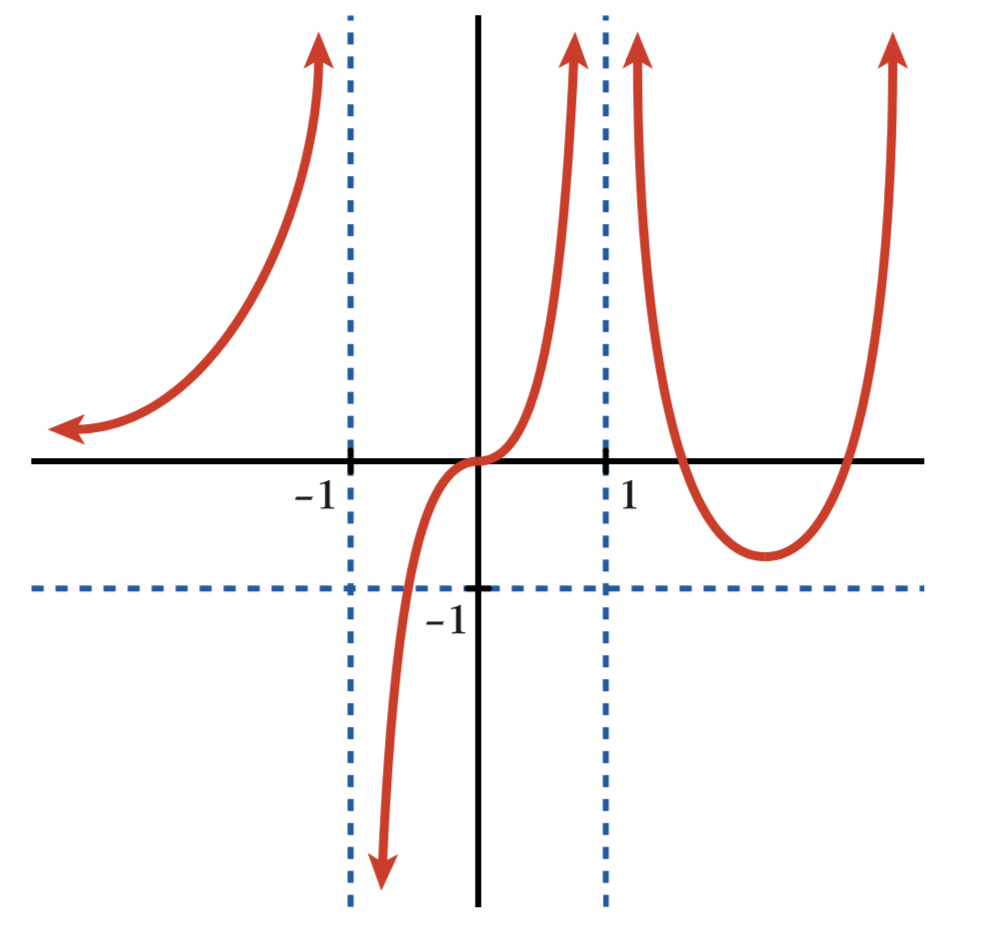
\includegraphics[width=5.2cm]{grafica1.jpg}
  \task $g(x)$:\par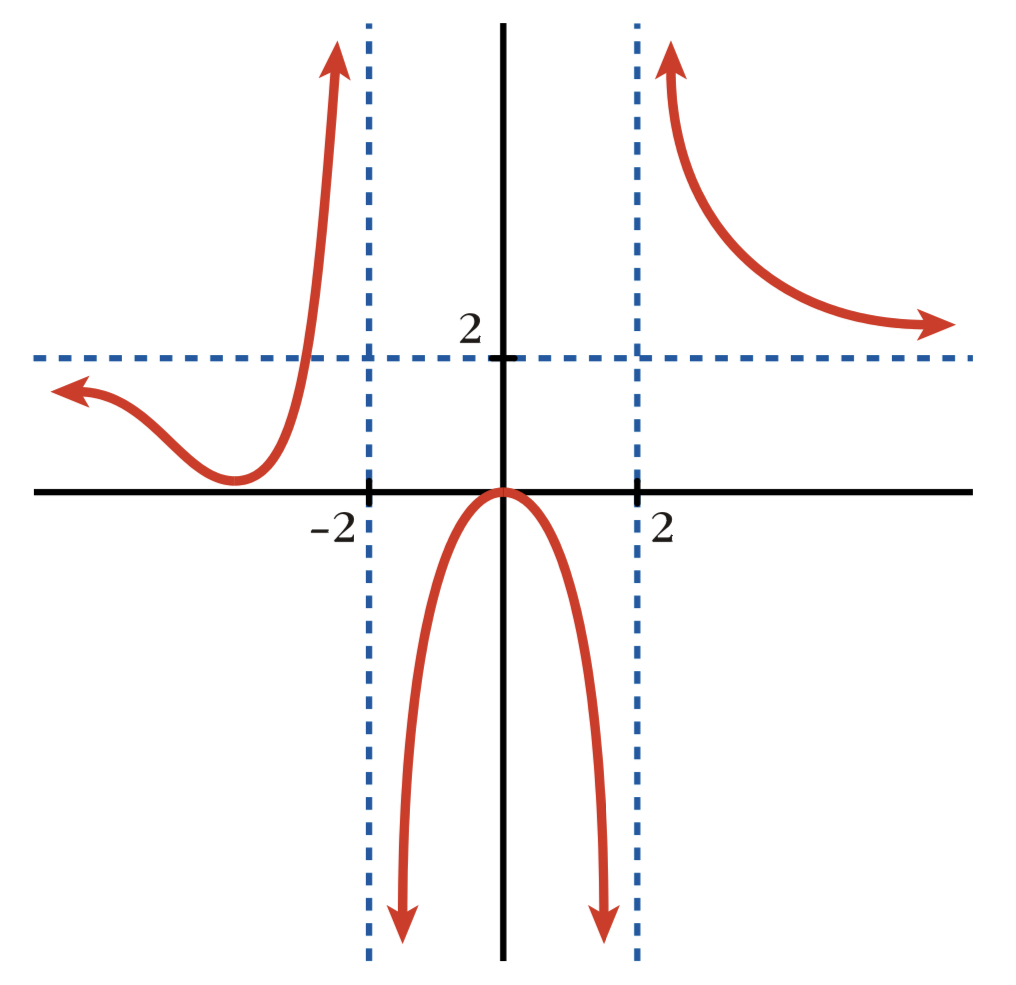
\includegraphics[width=5.2cm]{grafica2.jpg}
\end{tasks}\recorda{Para $x\to+\infty$ mira el \textbf{extremo derecho} de la gráfica; para $x\to-\infty$, el \textbf{extremo izquierdo}. Las rectas discontinuas son asíntotas.}

\ex{2} Lee en cada gráfica el límite cuando $x\to+\infty$ y cuando $x\to-\infty$. Fíjate bien en el dominio de cada función:\begin{tasks}(3)
  \task \begin{tikzpicture}[scale=0.42,baseline=(current bounding box.center)]\begin{scope}\draw[muted!30,very thin] (-1,-3) grid (5,2);\draw[-latex,thick] (-1,0)--(5.4,0);\draw[-latex,thick] (0,-3)--(0,2.4);\clip (-1,-3) rectangle (5,2);\draw[accent,line width=1.5pt,smooth,samples=90,domain=0.05:5] plot (\x,{ln(\x)});\node[below,font=\scriptsize] at (1,0) {$1$};\node[left,font=\scriptsize] at (0,1) {$1$};\end{scope}\end{tikzpicture}
  \task \begin{tikzpicture}[scale=0.42,baseline=(current bounding box.center)]\begin{scope}\draw[muted!30,very thin] (-4,-1) grid (5,3);\draw[-latex,thick] (-4,0)--(5.4,0);\draw[-latex,thick] (0,-1)--(0,3.4);\clip (-4,-1) rectangle (5,3);\draw[accent,line width=1.5pt,smooth,samples=90,domain=-3:5] plot (\x,{sqrt(\x+3)});\fill[accent] (-3,0) circle (0.17);\node[below,font=\scriptsize] at (-3,0) {$-3$};\node[below,font=\scriptsize] at (1,0) {$1$};\end{scope}\end{tikzpicture}
  \task \begin{tikzpicture}[scale=0.42,baseline=(current bounding box.center)]\begin{scope}\draw[muted!30,very thin] (-3,-1) grid (3,3);\draw[-latex,thick] (-3,0)--(3.4,0);\draw[-latex,thick] (0,-1)--(0,3.4);\clip (-3,-1) rectangle (3,3);\draw[accent,line width=1.5pt] (2,0) arc (0:180:2);\fill[accent] (-2,0) circle (0.17);\fill[accent] (2,0) circle (0.17);\node[below,font=\scriptsize] at (-2,0) {$-2$};\node[below,font=\scriptsize] at (2,0) {$2$};\end{scope}\end{tikzpicture}
\end{tasks}

\ex{1} Calcula los límites siguientes:\begin{tasks}(4)
  \task $\displaystyle\lim_{x\to +\infty}(3x^4-2x+7)$
  \task $\displaystyle\lim_{x\to -\infty}(-x^3+4x^2)$
  \task $\displaystyle\lim_{x\to -\infty}(2x^5-x^2)$
  \task $\displaystyle\lim_{x\to +\infty}(5-2x^2)$
\end{tasks}\recorda{El límite de un polinomio cuando $x\to\pm\infty$ es el de su \textbf{término de mayor grado}. Cuidado con el signo: $(-\infty)^{\text{par}}=+\infty$ y $(-\infty)^{\text{impar}}=-\infty$.}

\ex{1} Calcula comparando los grados del numerador y del denominador:\begin{tasks}(3)
  \task $\displaystyle\lim_{x\to +\infty}\dfrac{2x^3-x}{5x^3+4}$
  \task $\displaystyle\lim_{x\to +\infty}\dfrac{x^2+1}{x^3-2}$
  \task $\displaystyle\lim_{x\to -\infty}\dfrac{4x^4-x}{3x^2+1}$
  \task $\displaystyle\lim_{x\to -\infty}\dfrac{1-3x^2}{x+2}$
  \task $\displaystyle\lim_{x\to +\infty}\dfrac{7x-2}{3-x}$
  \task $\displaystyle\lim_{x\to +\infty}\dfrac{x^5}{100x^4+1}$
\end{tasks}\recorda{$\displaystyle\lim_{x\to\pm\infty}\frac{P(x)}{Q(x)}=\lim_{x\to\pm\infty}\frac{a_nx^n}{b_mx^m}$: \ si $n>m$, $\pm\infty$; \ si $n=m$, $\frac{a_n}{b_m}$; \ si $n<m$, $0$.}

\ex{2} Calcula los límites siguientes con raíces y exponenciales:\begin{tasks}(3)
  \task $\displaystyle\lim_{x\to +\infty}\dfrac{\sqrt{9x^2+1}}{2x-5}$
  \task $\displaystyle\lim_{x\to +\infty}\dfrac{\sqrt{x^3+x}}{x+4}$
  \task $\displaystyle\lim_{x\to +\infty}\dfrac{\sqrt[3]{8x^3-1}}{x}$
  \task $\displaystyle\lim_{x\to -\infty}\left(3^x+1\right)$
  \task $\displaystyle\lim_{x\to -\infty}0{,}4^{x}$
  \task $\displaystyle\lim_{x\to +\infty}\left(\tfrac{5}{2}\right)^{-x}$
\end{tasks}

\ex{3} Calcula $\displaystyle\lim_{x\to +\infty}\dfrac{6x+1}{\sqrt{4x^2+3}}$ y $\displaystyle\lim_{x\to -\infty}\dfrac{6x+1}{\sqrt{4x^2+3}}$. ¿Por qué no dan lo mismo?

\ex{3} \textbf{Repaso.} Calcula los límites siguientes. Cuidado con el signo de $x$ cuando $x\to-\infty$ y con el dominio de cada función:\begin{tasks}(2)
  \task $\displaystyle\lim_{x\to -\infty}\dfrac{\sqrt{x^4+1}}{2x^2-1}$
  \task $\displaystyle\lim_{x\to -\infty}\dfrac{\sqrt{x^2-5x+3}}{3x-2}$
  \task $\displaystyle\lim_{x\to -\infty}\left(\sqrt{x+1}-\sqrt{x+2}\right)$
  \task $\displaystyle\lim_{x\to -\infty}\dfrac{\sqrt{x^3-5x+3}}{x^2-2x}$
\end{tasks}


% =====================================================
\seccio{2}{Comparación de infinitos}

\ex{1} Ordena de menor a mayor orden de infinito (cuando $x\to+\infty$): \quad $x^3,\ \ 2^x,\ \ \ln x,\ \ \sqrt{x},\ \ e^x,\ \ x^{10}$.\recorda{Cuando $x\to+\infty$: \ logaritmos $\ll$ potencias $\ll$ exponenciales. Entre potencias gana el exponente mayor y entre exponenciales, la base mayor.}

\ex{2} Calcula los límites siguientes comparando infinitos:\begin{tasks}(3)
  \task $\displaystyle\lim_{x\to +\infty}\dfrac{x^3}{e^x}$
  \task $\displaystyle\lim_{x\to +\infty}\dfrac{2^x+x^4}{3\cdot2^x}$
  \task $\displaystyle\lim_{x\to +\infty}\dfrac{\ln x}{x^2}$
  \task $\displaystyle\lim_{x\to +\infty}\left(x^{10}-1{,}5^x\right)$
  \task $\displaystyle\lim_{x\to +\infty}\dfrac{e^x}{x^5+x}$
  \task $\displaystyle\lim_{x\to +\infty}\dfrac{3^x+2^x}{3^x-x^2}$
\end{tasks}


% =====================================================
\seccio{3}{Indeterminaciones}

\ex{2} Indeterminación $\infty-\infty$ con fracciones:\begin{tasks}(3)
  \task $\displaystyle\lim_{x\to +\infty}\left(\dfrac{x^2}{x+1}-x\right)$
  \task $\displaystyle\lim_{x\to +\infty}\left(\dfrac{2x^2+1}{x-1}-2x\right)$
  \task $\displaystyle\lim_{x\to +\infty}\left(\dfrac{x^3}{x^2+1}-\dfrac{x^2}{x+1}\right)$
\end{tasks}\recorda{Si la indeterminación $\infty-\infty$ viene de una resta de fracciones, \textbf{hacemos la resta} con denominador común y calculamos el límite del resultado.}

\ex{2} Indeterminación $\infty-\infty$ con raíces:\begin{tasks}(2)
  \task $\displaystyle\lim_{x\to +\infty}\left(\sqrt{x^2+8x}-x\right)$
  \task $\displaystyle\lim_{x\to +\infty}\left(\sqrt{4x^2+x}-2x\right)$
  \task $\displaystyle\lim_{x\to +\infty}\left(\sqrt{x^2+3x}-\sqrt{x^2-x}\right)$
  \task $\displaystyle\lim_{x\to +\infty}\left(\sqrt{x^2+1}-3x\right)$
\end{tasks}\recorda{Multiplicamos y dividimos por el \textbf{conjugado}: $(\sqrt A-B)(\sqrt A+B)=A-B^2$. Antes, comprueba si los términos principales se cancelan: si no lo hacen, no hace falta el conjugado.}

\ex{2} Indeterminación $1^{\infty}$:\begin{tasks}(3)
  \task $\displaystyle\lim_{x\to +\infty}\left(1+\dfrac5x\right)^{x}$
  \task $\displaystyle\lim_{x\to +\infty}\left(\dfrac{x+2}{x-1}\right)^{2x}$
  \task $\displaystyle\lim_{x\to +\infty}\left(\dfrac{2x-1}{2x+3}\right)^{x+1}$
  \task $\displaystyle\lim_{x\to +\infty}\left(\dfrac{x^2+3}{x^2-1}\right)^{x^2}$
  \task $\displaystyle\lim_{x\to +\infty}\left(\dfrac{3x+1}{x+2}\right)^{x}$
  \task $\displaystyle\lim_{x\to -\infty}\left(\dfrac{x-4}{x}\right)^{3x}$
\end{tasks}\recorda{Si $\lim f(x)=1$ y $\lim g(x)=\pm\infty$: \ $\lim f(x)^{g(x)}=e^{\lim\,(f(x)-1)\cdot g(x)}$. Si la base no tiende a 1, no hay indeterminación.}

\ex{2} Indeterminación $\frac{\infty}{\infty}$ con raíces:\begin{tasks}(2)
  \task $\displaystyle\lim_{x\to +\infty}\dfrac{\sqrt{x^2+5}+3x}{2x-1}$
  \task $\displaystyle\lim_{x\to +\infty}\dfrac{\sqrt{x^4+1}-x}{x^2+3}$
\end{tasks}

\ex{2} \pau{Aragón, EvAU extraordinaria 2020} Dada la función\[f(x)=\begin{cases}\dfrac{3}{x+1}&\text{si }x<-1\\[3pt]x^3-4x^2+2x-10&\text{si }-1\leq x\leq4\\[3pt]\sqrt{4x^2-7x}-2x&\text{si }x>4\end{cases}\]calcula $\displaystyle\lim_{x\to+\infty}f(x)$. (La continuidad de esta función se pide en la sección 6.)

\ex{2} \pau{Islas Baleares, PBAU extraordinaria 2021} El número de individuos, en millones, de una población viene determinado por la función $P(t)=\dfrac{2+t+t^2}{t^2+2t+1}$, donde $t\geq0$ mide el número de años transcurridos.\begin{tasks}(1)
  \task ¿Cuál es la población inicial ($t=0$) y la población después de 5 años?
  \task ¿A partir de qué momento la población será inferior a un millón de individuos?
  \task Con el paso de los años, ¿hacia qué valor tenderá el número de individuos de la población?
\end{tasks}

\ex{2} \pau{Castilla y León, EBAU junio 2017} El beneficio, en miles de euros, de una empresa transcurridos $x$ meses es\[f(x)=\begin{cases}20x^2-20x+32&\text{si }0<x\leq1\\[3pt]\dfrac{90x-45}{x+8}+27&\text{si }x>1\end{cases}\]Determina el beneficio de la empresa a muy largo plazo.

\ex{3} \pau{Cataluña, PAU septiembre 2018} Se sabe que la función $f(x)=\dfrac{ax+b}{cx+1}$ pasa por el punto $(2,-5)$ y que las rectas $x=1$ e $y=2$ son, respectivamente, su asíntota vertical y horizontal. Calcula $a$, $b$ y $c$.

\ex{2} \textbf{Repaso.} Calcula los límites siguientes cuando $x\to-\infty$. Antes de nada, comprueba si de verdad hay una indeterminación:\begin{tasks}(2)
  \task $\displaystyle\lim_{x\to -\infty}\left(\dfrac{x^2}{x-3}-\dfrac{x^2}{5-x}\right)$
  \task $\displaystyle\lim_{x\to -\infty}\left(\dfrac{3x^2}{x+1}-\dfrac{x^3}{x^2+1}\right)$
  \task $\displaystyle\lim_{x\to -\infty}\left(\sqrt{x^2+x}-\sqrt{x^2+1}\right)$
  \task $\displaystyle\lim_{x\to -\infty}\left(2x-\sqrt{x^2+x}\right)$
\end{tasks}

\ex{2} \textbf{Repaso.} Calcula:\begin{tasks}(3)
  \task $\displaystyle\lim_{x\to -\infty}\left(\dfrac{3x+4}{2x+5}\right)^{x-1}$
  \task $\displaystyle\lim_{x\to -\infty}\left(\dfrac{2x+1}{2x-1}\right)^{x-1}$
  \task $\displaystyle\lim_{x\to -\infty}\left(\dfrac{x^2+1}{x^2-1}\right)^{\frac{x^2-4}{x-1}}$
\end{tasks}


% =====================================================
\seccio{4}{Límites en un punto e indeterminación 0/0}

\ex{1} Vuelve a las gráficas de $f$ y $g$ del ejercicio \ref{ex:g1} y calcula los límites siguientes, estudiando los límites laterales cuando sea necesario:\begin{tasks}(3)
  \task $\displaystyle\lim_{x\to -1}f(x)$
  \task $\displaystyle\lim_{x\to 1}f(x)$
  \task $\displaystyle\lim_{x\to 0}f(x)$
  \task $\displaystyle\lim_{x\to -2}g(x)$
  \task $\displaystyle\lim_{x\to 2}g(x)$
  \task $\displaystyle\lim_{x\to 0}g(x)$
\end{tasks}

\ex{1} \label{ex:g4}Dada la gráfica de la función $f(x)$, calcula $\displaystyle\lim_{x\to+\infty}f(x)$, $\displaystyle\lim_{x\to-\infty}f(x)$ y $\displaystyle\lim_{x\to0}f(x)$.\par\smallskip{\centering \begin{tikzpicture}[scale=0.5,baseline=(current bounding box.center)]\begin{scope}\draw[muted!30,very thin] (-4,-3) grid (4,4);\draw[-latex,thick] (-4,0)--(4.4,0);\draw[-latex,thick] (0,-3)--(0,4.4);\clip (-4,-3) rectangle (4,4);\draw[accent,line width=1.5pt,smooth,samples=90,domain=-3.46:0] plot (\x,{\x*\x/2-2});\draw[accent,line width=1.5pt,smooth,samples=90,domain=0:4] plot (\x,{1+1/(\x+1)});\draw[teal,dashed] (-4,1)--(4,1);\filldraw[fill=white,draw=accent,line width=1.1pt] (0,-2) circle (0.17);\fill[accent] (0,2) circle (0.17);\node[below,font=\scriptsize] at (1,0) {$1$};\node[left,font=\scriptsize] at (0,1) {$1$};\end{scope}\end{tikzpicture}\par}

\ex{1} Calcula los límites siguientes. Cuando sea necesario, estudia los límites laterales:\begin{tasks}(3)
  \task $\displaystyle\lim_{x\to 2}(x^3-2x+1)$
  \task $\displaystyle\lim_{x\to -1}\dfrac{x^2+3}{x-1}$
  \task $\displaystyle\lim_{x\to 3}\dfrac{2x}{x-3}$
  \task $\displaystyle\lim_{x\to 0}\dfrac{x-1}{x^2}$
  \task $\displaystyle\lim_{x\to 4^+}\sqrt{x-4}$
  \task $\displaystyle\lim_{x\to 1}\dfrac{x+1}{(x-1)^3}$
\end{tasks}\recorda{Si al sustituir sale $\frac{k}{0}$ con $k\neq0$, el límite es infinito: estudiamos el signo por la izquierda y por la derecha.}

\ex{2} Calcula $\displaystyle\lim_{x\to2}f(x)$ y $\displaystyle\lim_{x\to-1}f(x)$, si existen, para\[f(x)=\begin{cases}x^2-3&\text{si }x<-1\\[3pt]2x&\text{si }-1\leq x<2\\[3pt]\dfrac{8}{x}&\text{si }x\geq2\end{cases}\]

\ex{2} Resuelve las indeterminaciones $\frac00$ factorizando:\begin{tasks}(3)
  \task $\displaystyle\lim_{x\to 3}\dfrac{x^2-5x+6}{x^2-9}$
  \task $\displaystyle\lim_{x\to 2}\dfrac{x^3-8}{x-2}$
  \task $\displaystyle\lim_{x\to 1}\dfrac{x^3-x^2-x+1}{x^2-1}$
  \task $\displaystyle\lim_{x\to 1}\dfrac{x^4-1}{x^2-x}$
  \task $\displaystyle\lim_{x\to -3}\dfrac{x^2+3x}{x^2+6x+9}$
  \task $\displaystyle\lim_{x\to 4}\dfrac{\sqrt{x+5}-3}{x-4}$
\end{tasks}\recorda{Si $P(a)=Q(a)=0$, ambos son divisibles por $(x-a)$: factorizamos (Ruffini, identidades notables, factor común), simplificamos y volvemos a sustituir.}

\ex{2} \textbf{Repaso.} Calcula los límites siguientes:\begin{tasks}(3)
  \task $\displaystyle\lim_{x\to 3}\dfrac{x-3}{x^3-5x^2+3x+9}$
  \task $\displaystyle\lim_{x\to 2}\left(\dfrac{2}{x-2}-\dfrac{x+1}{x^2-2x}\right)$
  \task $\displaystyle\lim_{x\to 2}\dfrac{x^2+x-6}{x^2-x-1}$
  \task $\displaystyle\lim_{x\to 2}\left(\dfrac{x+2}{2x}\right)^{\frac{x^2-4}{x-1}}$
  \task $\displaystyle\lim_{x\to -1}\dfrac{x^3-2x^2+2x+5}{x^2-6x-7}$
  \task $\displaystyle\lim_{x\to 2}\dfrac{2x^2+x-10}{x^3-3x^2+4}$
\end{tasks}


% =====================================================
\seccio{5}{Continuidad en un punto. Funciones racionales}

\ex{1} Vuelve a la gráfica de $f$ del ejercicio \ref{ex:g1}. ¿Existe $\displaystyle\lim_{x\to1}f(x)$? ¿Por qué la función no es continua en $x=1$? Y la función del ejercicio \ref{ex:g4}, ¿es continua en $x=0$? Justifica las respuestas.

\ex{1} Estudia la continuidad de cada función en el punto indicado y, si es discontinua, di de qué tipo es:\begin{tasks}(2)
  \task $f(x)=\dfrac{x^2-4}{x+2}$ \ en $x=-2$
  \task $g(x)=\dfrac{3}{x-4}$ \ en $x=4$
  \task $h(x)=\begin{cases}x^2+1&\text{si }x<0\\x+1&\text{si }x\geq0\end{cases}$ \ en $x=0$
  \task $k(x)=\begin{cases}2x&\text{si }x\leq1\\x^2+3&\text{si }x>1\end{cases}$ \ en $x=1$
\end{tasks}\recorda{$f$ es continua en $a$ si: \ 1) $\exists f(a)$; \ 2) $\exists\lim_{x\to a}f(x)$; \ 3) $\lim_{x\to a}f(x)=f(a)$. Tipos: evitable, de salto finito, de salto infinito y asintótica.}

\ex{2} Estudia la continuidad de $f(x)=\dfrac{x^2+x-2}{x^2-4x+3}$ y clasifica sus discontinuidades.

\ex{2} \pau{Cantabria, EBAU julio 2019} Sea la función $f(x)=\dfrac{x^2-x-12}{x^2-2x-15}$. ¿En qué puntos es discontinua? ¿Se puede definir de nuevo esta función para evitar alguna discontinuidad?

\ex{2} \pau{Cantabria, EBAU ordinaria 2020} Dada la función $f(x)=\dfrac{2x+4}{x^2+5x+6}$:\begin{tasks}(1)
  \task ¿En qué puntos es discontinua?
  \task ¿Se puede definir de nuevo la función para evitar alguna discontinuidad?
  \task Calcula los dos límites laterales en $x=-3$ e interpreta gráficamente qué ocurre alrededor de este valor.
\end{tasks}

\ex{2} \pau{Navarra, EvAU ordinaria 2021} Estudia la continuidad de la función $f(x)=\dfrac{x^2+4x+3}{2x-2}$ y, si procede, indica el tipo de discontinuidad.


% =====================================================
\seccio{6}{Continuidad de funciones a trozos}

\ex{1} \pau{Navarra, EvAU extraordinaria 2021} Estudia la continuidad de la función\[f(x)=\begin{cases}x^2-2x&\text{si }x\leq2\\[3pt]-x^2+6x-8&\text{si }x>2\end{cases}\]\recorda{Primero estudiamos la continuidad de cada trozo por separado y después miramos los puntos donde la función se parte: $f(a)$, $\lim_{x\to a^-}f$ y $\lim_{x\to a^+}f$.}

\ex{2} \pau{Castilla y León, EBAU septiembre 2017} Estudia razonadamente la continuidad de\[f(x)=\begin{cases}\dfrac{1}{4-x^2}&\text{si }0<x<2\\[3pt]2x&\text{si }2\leq x<4\end{cases}\]

\ex{2} \pau{Madrid, EvAU junio 2018} Estudia si es continua en $x=2$ la función\[f(x)=\begin{cases}\dfrac{x+2}{x-1}&\text{si }x\leq2\\[3pt]\dfrac{3x^2-2x}{x+2}&\text{si }x>2\end{cases}\]Estudia también su continuidad en todo $\mathbb R$.

\ex{2} \pau{Madrid, EvAU julio 2018} Determina el dominio de $f$ y estudia su continuidad:\[f(x)=\begin{cases}x^3+2e^x&\text{si }x<0\\[3pt]\dfrac{2}{3+x}&\text{si }x\geq0\end{cases}\]

\ex{2} \pau{Aragón, EvAU extraordinaria 2020} Estudia la continuidad de\[f(x)=\begin{cases}\dfrac{3}{x+1}&\text{si }x<-1\\[3pt]x^3-4x^2+2x-10&\text{si }-1\leq x\leq4\\[3pt]\sqrt{4x^2-7x}-2x&\text{si }x>4\end{cases}\]

\ex{3} \pau{Madrid, EvAU junio 2019} Analiza la continuidad de la función en todo su dominio según los valores de $k$:\[f(x)=\begin{cases}e^x+k&\text{si }x\leq0\\[3pt]1-x^2&\text{si }0<x\leq3\\[3pt]\dfrac{1}{x-3}&\text{si }x>3\end{cases}\]

\ex{2} \textbf{Repaso.} Estudia la continuidad de las funciones siguientes en su dominio:\begin{tasks}(2)
  \task $f(x)=\begin{cases}1&\text{si }x<0\\[3pt]x+1&\text{si }0<x<1\\[3pt]x^2-2x&\text{si }1\leq x\end{cases}$
  \task $g(x)=\begin{cases}3x-x^2&\text{si }x\leq3\\[3pt]x-3&\text{si }3<x<6\\[3pt]0&\text{si }x\geq6\end{cases}$
\end{tasks}


% =====================================================
\seccio{7}{Funciones a trozos con parámetros}

\ex{1} \pau{Madrid, EvAU septiembre 2017} Calcula el valor del parámetro real $a$ para que $f$ sea continua en todo su dominio:\[f(x)=\begin{cases}ax+1&\text{si }x<-1\\[3pt]x^2+x-2&\text{si }x\geq-1\end{cases}\]\recorda{Igualamos los límites laterales (y $f(a)$) en cada punto donde cambia la expresión. Con dos parámetros, obtenemos un sistema.}

\ex{1} \pau{Andalucía, PEvAU junio 2019} Determina el valor del parámetro $a$ para que $f$ sea continua en todo su dominio:\[f(x)=\begin{cases}\dfrac{1}{x-1}&\text{si }x<0\\[3pt]x^2+a&\text{si }x\geq0\end{cases}\]

\ex{2} \pau{Castilla-La Mancha, EvAU extraordinaria 2020} Halla el valor de $t$ para el que es continua en $x=0$ la función\[f(x)=\begin{cases}x-t&\text{si }x\leq0\\[3pt](x-t)^2-5(x+t)+4&\text{si }x>0\end{cases}\]

\ex{2} \pau{Castilla-La Mancha, EvAU extraordinaria 2020} Se considera la función \[f(x)=\begin{cases}-4x+4&\text{si }x\leq c\\[3pt]x^2-4x&\text{si }x>c\end{cases}\]¿Para qué valores de $c$ es continua en $x=c$?

\ex{2} \pau{Islas Baleares, PBAU extraordinaria 2021} Calcula los valores de $a$ para que $f(x)$ sea continua:\[f(x)=\begin{cases}-4x+a&\text{si }x\leq-2\\[3pt]x^2-5&\text{si }-2<x<1\\[3pt]-7x+3&\text{si }x\geq1\end{cases}\]

\ex{2} \pau{Cataluña, PAU septiembre 2018} Halla el valor de $a$ y $b$ para que la función sea continua para todos los números reales:\[f(x)=\begin{cases}2x+3&\text{si }x\leq-1\\[3pt]ax+b&\text{si }-1<x<2\\[3pt]x^2&\text{si }x\geq2\end{cases}\]

\ex{3} \pau{Aragón, EvAU septiembre 2018} Calcula $a$ y $b$ sabiendo que $f$ es continua en todos los puntos:\[f(x)=\begin{cases}ax+1&\text{si }x<-2\\[3pt]\dfrac{x+b}{x^2+1}&\text{si }-2\leq x<0\\[3pt]x^3-9x^2+24x+4&\text{si }x\geq0\end{cases}\]

\ex{3} \pau{Cantabria, EBAU ordinaria 2020} Determina los valores de $a$ y $b$ para los que la función es continua en $x=-1$ y en $x=3$:\[f(x)=\begin{cases}ax^2+2x-1&\text{si }x\leq-1\\[3pt]x^2-5&\text{si }-1<x\leq3\\[3pt]\dfrac{b+x}{3x-2}&\text{si }x>3\end{cases}\]

\ex{3} \pau{Cantabria, EBAU julio 2019} Determina los valores de $a$ y $b$ para los que la función es continua en $x=-2$ y en $x=0$:\[f(x)=\begin{cases}-6x+3&\text{si }-4<x<-2\\[3pt]x^2+ax+5&\text{si }-2\leq x<0\\[3pt]\dfrac{x+15}{x+b}&\text{si }0\leq x<3\end{cases}\]

\ex{2} \textbf{Repaso.} Dada la función\[f(x)=\begin{cases}-\dfrac{1}{x^2}&\text{si }x<1\\[3pt]x^2+ax&\text{si }x\geq1\end{cases}\]\begin{tasks}(1)
  \task Calcula el valor de $a$ para que la función sea continua en $x=1$.
  \task Para el valor de $a$ obtenido, estudia la continuidad de la función en su dominio.
\end{tasks}

\ex{3} \textbf{Repaso.} Calcula los valores de los parámetros $a$ y $b$ para que las funciones siguientes sean continuas en su dominio:\begin{tasks}(2)
  \task $f(x)=\begin{cases}\dfrac{1}{x^2}+a&\text{si }x\leq-1\\[3pt]3x^2+4&\text{si }-1<x<1\\[3pt]-x^2+b&\text{si }x\geq1\end{cases}$
  \task $g(x)=\begin{cases}-2x+a&\text{si }x\leq-2\\[3pt]x^2-5&\text{si }-2<x<1\\[3pt]bx+3&\text{si }1\leq x\end{cases}$
\end{tasks}


% =====================================================
\seccio{8}{Asíntotas}

\ex{1} Calcula las asíntotas verticales y horizontales de las funciones siguientes. En cada asíntota vertical, estudia los límites laterales:\begin{tasks}(3)
  \task $f(x)=\dfrac{3x+2}{x-1}$
  \task $f(x)=\dfrac{4}{x^2-16}$
  \task $f(x)=\dfrac{2x^2}{x^2+3}$
  \task $f(x)=\dfrac{x+1}{(x-2)^2}$
  \task $f(x)=\dfrac{1-x^2}{x^2+x-2}$
  \task $f(x)=\dfrac{x^2-9}{x+3}$
\end{tasks}\recorda{AV $x=a$: si $\lim_{x\to a^\pm}f(x)=\pm\infty$ (en una racional, donde el límite da $\frac{k}{0}$, $k\neq0$; si da $\frac00$, simplificamos). AH $y=b$: si $\lim_{x\to\pm\infty}f(x)=b$.}

\ex{2} Calcula las asíntotas horizontales de las funciones siguientes, cuando $x\to+\infty$ y cuando $x\to-\infty$:\begin{tasks}(3)
  \task $f(x)=3^x+2$
  \task $f(x)=4-e^{-x}$
  \task $f(x)=\dfrac{6\cdot2^x}{2^x+1}$
\end{tasks}

\ex{2} Calcula las asíntotas oblicuas por el método del cociente y también las verticales. Estudia la posición de la gráfica respecto de la asíntota oblicua:\begin{tasks}(2)
  \task $f(x)=\dfrac{x^2+2}{x-1}$
  \task $f(x)=\dfrac{3x^2-x}{x+2}$
  \task $f(x)=\dfrac{x^3+2}{x^2}$
  \task $f(x)=\dfrac{-x^2+4x}{x-3}$
\end{tasks}\recorda{Si grado $P=$ grado $Q+1$, dividimos: $P(x)=Q(x)\cdot C(x)+R(x)\Rightarrow f(x)=C(x)+\dfrac{R(x)}{Q(x)}$. La asíntota oblicua es $y=C(x)$ y el signo de $\frac{R(x)}{Q(x)}$ nos dice si la gráfica queda por encima o por debajo.}

\ex{2} Calcula todas las asíntotas de las funciones siguientes:\begin{tasks}(3)
  \task $f(x)=\dfrac{x^2-x}{x^2-1}$
  \task $f(x)=\dfrac{x^3}{x^2-4}$
  \task $f(x)=\dfrac{x^3+1}{x-1}$
\end{tasks}

\ex{3} Dada la función $f(x)=\dfrac{ax^2+1}{x+b}$:\begin{tasks}(1)
  \task Calcula $a$ y $b$ para que $f$ tenga una asíntota vertical en $x=-2$ y una asíntota oblicua de pendiente $3$.
  \task Para estos valores, ¿cuál es la ecuación de la asíntota oblicua?
\end{tasks}

\ex{2} Las ventas de un nuevo producto, en miles de unidades, $t$ meses después del lanzamiento vienen dadas por $V(t)=\dfrac{50t}{t+4}$, con $t\geq0$.\begin{tasks}(1)
  \task Calcula las ventas a los 6 meses.
  \task Calcula $\displaystyle\lim_{t\to+\infty}V(t)$. ¿Qué asíntota tiene la función? Interprétala en el contexto del problema.
\end{tasks}

\vfill
\begin{center}\color{muted}\small\faCheckCircle[regular]\ \ ¡Ánimo! Comprueba tus resultados con la calculadora de límites de los apuntes interactivos.\end{center}

\end{document}
